%
% The points that I want to cover are the following:
%
% \begin{itemize}
%   \item Building the network from the bioinformatics data and clustering.
%   \item Manipulation of the network: translation and scaling.
%   \item Locomotion and ergonomics used in the VR environment.
%   \item Changing from the blood network to the biopsy network and viceversa.
%   \item Filtering genes in the network using gene sets that represent signatures of cellular pathways which are often dis-regulated in cancer.
% \end{itemize}

%In order to explore the network, several features have been implemented with the purpose of enhance the experience of the visualization process. For example the user has the possibility to move around the network by teleporting to a different place. It is also possible to translate the network and scale it, allowing the user have a better view of the data. The user can also point at a node using the controller to show the name corresponding to that gene or node. Another feature is about entering into a menu where the user can filter the network according to gene sets that represent signatures of cellular pathways which are often dis-regulated in cancer. And finally it is possible also to switch the network from a blood dataset to a biopsy dataset and viceversa.

%The genes nodes in the network and are represented as squared dots and the relationships are represented with lines between them. In Figure \ref{fig:mixt_vr} we can see an example of the application running.

MIxT VR is a virtual reality application for the interactive visualization of large-scale networks in a 3D space. The networks are represented using nodes and connections between them. In order to explore the data, the user can walk around, scale the network, move it around, filter the nodes using a 2D interface and also interact with the nodes to get more information about them. In Figure \ref{fig:mixt_vr} we can see an example of the application running.

MIxT VR works with a dataset that contains the information of the nodes and relationships of the network. This dataset needs to be obtained from an external source or application. Once we have our dataset we can load it to the application and then run MIxT VR using a Head Mounted Display or HMD for VR. Finally we can explore the network and interact with it to visualize the dataset in a VR experience.

The implementation of MIxT VR is done in Unity, a cross-platform game engine. This engine is used for a wide range of applications, especially for the development of videogames in 3D and 2D, VR applications and engineering solutions. The programming language used to develop the application inside Unity is C\#. We also used VRTK, a VR toolkit to build VR solutions in Unity. As for the VR hardware, we used an Oculus Quest headset. This type of headset is an oll-in-one HMD, which means that it doesn't need to be connected to a PC to run an application, it can be run inside the hardware of the headset itself. However during the development process, the headset needs to be connected to the PC and the application can be run directly from Unity.

For this chapter we will use dataset examples from MIxT to illustrate the concepts in this chapter. MIxT is a web application that is used for the visualization of bioinformatic data\cite{fjukstad_dumeaux_olsen_lund_hallett_bongo_2017}\cite{dumeaux_fjukstad_interactions_tumor_blood} and the datasets used here contain genetic information about a woman with breast cancer. There are in total 2 datasets, the first one is from a blood sample and the second one is from the tumor sample. In Figure \ref{fig:mixt_vr} we can see an example of the application running using the blood dataset from MIxT.

\begin{figure}[h!]
    \setlength{\tempheight}{15ex}
    \centering
    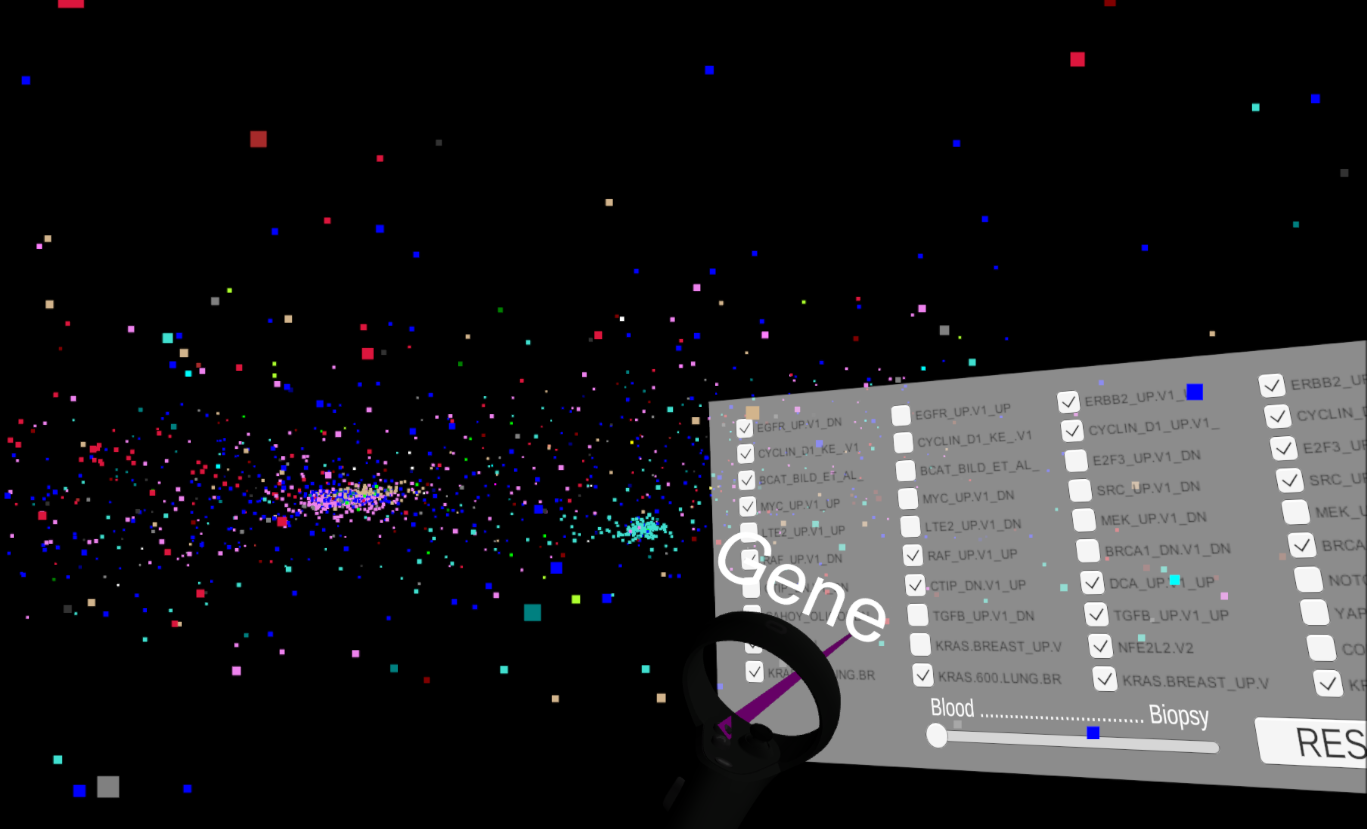
\includegraphics[width=\textwidth]{mixt_vr}
    \caption{MIxT VR. Example of the application running on a Oculus Quest.}
    \label{fig:mixt_vr}
\end{figure}

\section{Visualization and interaction with the network}
Virtual reality headsets offer a rich inmmersive experience. It's not only about inmersing the user into a 3D environment, but also giving the user the possibility to interact with the environment itself. This makes it possible to build complex VR applications where the user can do almost anything in a virtual world. Some exmaples of what it is possible to do in a VR application is for example moving around by teleporting to a different spot, grabbing objects, showing 2D menus and interact with it, etc. In this section we will explain the techniques that we have implemented to visualize and interact with the network. These techniques correspond to how the user can move around in the network and how the user can manipulate it.

Oculus Quest is an all-in-one VR hardware and so it doesn't need a PC nor wires to run the applications. Apart from the headset it comes with 2 controllers, one for each hand. These controlers have inputs as buttons, thumbsticks and triggers that can be used to activate actions in the VR application. Some of the inputs have been mapped to trigger different actions to interact with the network and the environment in MIxT VR. In Figure \ref{fig:oculus_quest_inputs} we can see which action correspond each input from the controllers.

\begin{figure}[h!]
    \centering%
    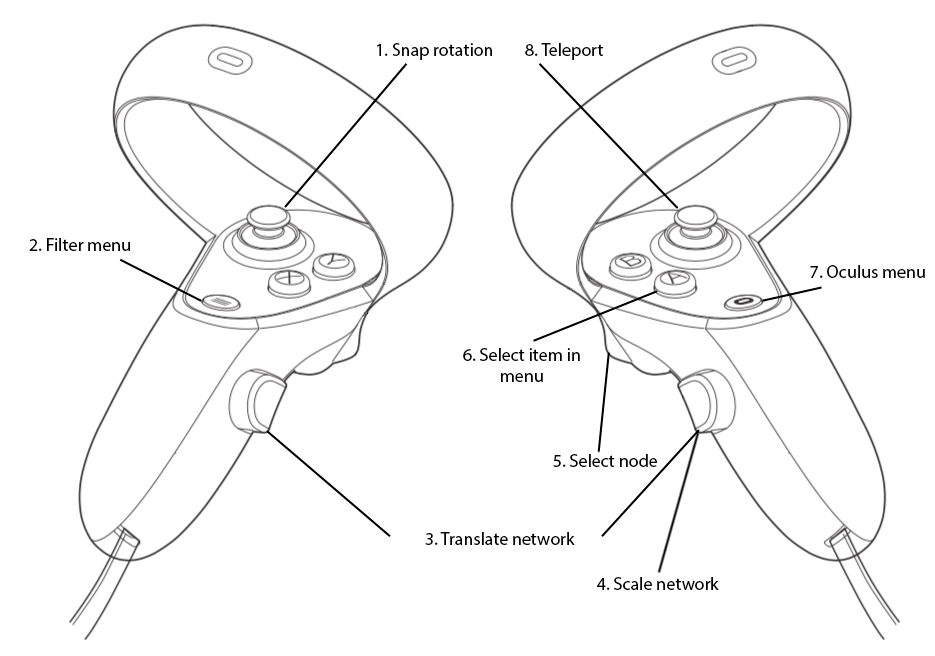
\includegraphics[width=\textwidth]{oculus_quest_inputs}
    \caption{Mapping of the Oculus Quest controllers for the different actions implemented in MIxT VR. 1. Snap rotation. 2. Filter menu. 3. Scale environment. 4. Translate environment. 5. Select item in menu. 6. Oculus menu. 7. Teleport.}
    \label{fig:oculus_quest_inputs}
\end{figure}%

\subsection{Locomotion}
How the player can move around the environment.

\subsection{Network manipulation}
Translation and scaling of the network for better visualization.

\section{Creation of the network in a 3D space}

\begin{table}[h!]
\centering
\begin{tabular}{ll}
\hline
category & genes          \\
brown   & ARHGAP30 FERMT3 ARHGAP25 CD53 PLEK IRF8 DOCK2\\
cyan  & SAFB MOB3A RAB35 ABR ASCC2 CDC37 ANKFY1 GLTSCR1\\
darkgrey  & RAB40C ZNF213 ZNF263 PIGQ RHBDF1 RAB11FIP3\\
darkorange  & TCEB1 MRPL13 ENY2 MTERF3 UBE2W WDYHV1\\
\hline
\end{tabular}
\caption{Fragment of the dataset with the categories and the genes belonging to each category from the biopsy sample.}
\label{tab:categories-data}
\end{table}

\begin{table}[h!]
\centering
\begin{tabular}{llll}
\hline
source & target & weight            & id          \\
AAMP   & ARGLU1 & 0.102486209330144 & AAMP-ARGLU1 \\
ACADM  & FOXN2  & 0.107506881676173 & ACADM-FOXN2 \\
ACADM  & MBNL1  & 0.12269622045714  & ACADM-MBNL1 \\
ACADM  & PPM1B  & 0.103496640767895 & ACADM-PPM1B \\
\hline
\end{tabular}
\caption{Fragment of the dataset used to build the network relationships of the blood sample.}
\label{tab:network-data}
\end{table}

\section{Filtering information in the network}
How the network is filtered.
